% !TEX root = ../main.tex

% Background section

\section{The Variational Bernstein von--Mises Theorem}

\paragraph{} We now present the Variational Bernstein von--Mises theorem. In this form, the BvM states that the VB posterior converges in total variation to the variational approximation to a normal distribution, i.e., the KL minimizer within the variational family to some normal. The proof of the theorem follows directly from four preceding lemmata. The notation for the rest of the report will be in the style of \cite{Wang:2019:VBVM}, with translatations from \cite{Asymptotics:2000} when necessary. As before, assume that there exists a true atomic value of the parameter $\theta_0$, and further suppose that the model also depends locally on a latent parameter $z$. That is, the model has density
\begin{equation}
\label{model}
\int p(x, z|\theta = \theta_0)dz 
\end{equation}
while each draw from the model implicitly carries a realization of the latent state. 
\subsection{VB Ideal}
Define the frequentist variational model to have likelihood
\begin{equation}
\ell_n(\theta; x) \propto \exp(M_n(\theta;x))
\end{equation}
then, the VB ideal $\pi^*(\theta|x)$ is the usual posterior density under this model. Denote the associated VB posterior distribution to be $\Pi^*$. Importantly, the frequentist variational model is typically misspecified for the true model in equation \ref{model}, since the maximum and expectation operators in equation (8) does not recover the model log-likelihood unless the local optimal $q_z$ recovers $p(z|x, \theta)$ exactly. As mentioned, a BvM result exists for model misspecification \cite{kleijn2012}, which will be applied in the result here. Recall that in Theorem \ref{bvm}, the posterior distributions were centered at $\theta_0$ and scaled by $\sqrt{n}$. We also define a similar transformation here:
\begin{equation}
\tilde{\theta} = \delta_n^{-1}(\theta - \theta_0) 
\end{equation}
for some diagonal matrix $\delta_n$. Then, we have the transformed VB ideal $\tilde{\Pi}$ with density:
\begin{equation}
\tilde{\pi}(\tilde{\theta}|x) = \pi^*(\theta_0 + \delta_n\tilde{\theta}|x) |det(\delta_n)|
\end{equation}
We will now briefly discuss the conditions of the variational BvM in the context of (A1) -- (A3) in the background section. For the rest of the report, assume the following conditions:
\begin{itemize}
	\item (VA1) (Prior Mass) The prior distribution has a density $p(\theta)$ that is continuous and positive on a neighbourhood of $\theta_0$. There exists a constant $M_p >0$ such that $|(\log p(c))''| \leq M_p e^{|c|^2}$ for all $c \in \bbR$. 
	\item (VA2) (Consistent Testability) For every $\epsilon > 0$, there exists a sequence of tests $\phi_n$ such that 
	$$
	\int \phi_n(x)p(x, z|\theta_0)dxdz
	$$
	$$
	\sup_{\theta: \|\theta-\theta_0\| \geq \epsilon} \int (1-\phi_n(x))\frac{\ell_n(\theta;x)}{\ell_n(\theta_0; x)}p(x,z|\theta_0) dxdz
	$$
	\item (VA3) (LAN) For every compact set $K \in \bbR^d$, there exists random vectors $\Delta_{n, \theta_0}$ bounded in probability and nonsingular matrices $V_{\theta_0}$ such that for $\delta_n \to 0$ a diagonal matrix, we have
	\begin{equation}
	\sup_{h\in K} |M_n(\theta + \delta_n h; x) - M_n(\theta; x) - h^T V_{\theta_0}\Delta_{n, \theta_0}' + \frac{1}{2}h^TV_{\theta_0}h| \to 0
	\end{equation}
	in probability under the 'true' data distribution $P_{\theta_0}$. Note the notation $\Delta_{n, \theta_0}'$ is slightly changed from \cite{Wang:2019:VBVM} to contrast with the standard (A3). $\Delta_{n, \theta_0}'$ plays the same role as $\Delta_{n, \theta_0}$ in the traditional BvM, but here it is only a bounded random vector while in Theorem \ref{bvm} it is exactly specified. 
\end{itemize}
Note that (VA1) and (A1) are almost equivalent conditions - there is only a mild technical addition on the hessian of the prior density that is true for most non-heavy tailed distributions. (VA3) is equivalent to (A3) by replacing the model with the frequentist variational model, and its truth is checked case-by-case by analyzing $M_n$. As mentioned, in the case where there are no local latent variables, (A3) corresponds to (VA3) exactly. There are conditions that may be checked for when the LAN expansions in (A3) and (VA3) have an exact correspondence, see (\cite{Wang:2019:VBVM}, section 3.4) for a detailed discussion. Connecting (VA2) and (A2) requires a bit more care. (VA2) roughly states that there exists a sequence of tests for identifying the events $\|\theta-\theta_0\| \geq \epsilon$ and $\theta = \theta_0$ given samples from the true model, assessed under the likelihood ratio of the misspecified variational model. This is shown to be equivalent to the testability condition in \cite{kleijn2012}, which implies the misspecified BvM. 
\begin{lemma}[Lemma 1, \cite{Wang:2019:VBVM}]
	\label{lem1}
	Under assumptions (VA1) -- (VA3), we have
	\begin{equation*}
		\|\tilde{\Pi} - N(\Delta_{n, \theta_0}', V^{-1}_{\theta_0}) \|_{TV}
	\end{equation*}
\end{lemma}

The proof of Lemma \ref{lem1} boils down to checking that assumption (VA2) implies the consistent testability condition for misspecified BvM (\cite{kleijn2012}, (2.3)), then applying this result to the rescaled VB ideal posterior. Notice that this is almost the statement in Theorem \ref{bvm}. The key difference is that we use $\Delta_{n, \theta_0}'$ and $V_{\theta_0}$ in place of the more specifically defined $\Delta_{n, \theta_0}$ and $I_{\theta_0}$.

\subsection{KL Minimizer of the VB Ideal}

\paragraph{} Recall that the VB ideal is highly complex and of little practical interest. To relate it to practical VI, a second variational approximation must be made to the VB ideal itself. Since the VB ideal is parametrized only by $\theta$, the mean-field family is just $Q^d$. Heuristically, the scaled VB ideal converges to a distribution with Normal spread, so from traditional asymptotics it is expected that the unscaled version converges instead to a point mass. We show that the variational approximation converges to the point mass at $\theta_0$, i.e., it is consistent.

\begin{lemma}[Lemma 2, \cite{Wang:2019:VBVM}]
	\label{lem2}
	Let $\delta_{\theta_0}$ be the dirac probability measure at $\theta_0$. Then, the following event occurs almost surely under the probability measure $P_{\theta_0}$:
	\begin{equation*}
	\arg\min_{Q^{d}} \text{KL}(q_{\theta}(\theta) \| \pi^*(\theta|x)) \to \delta_{\theta_0}
	\end{equation*}
	in distribution.
\end{lemma}

A heuristic sketch of the proof is that mean-field families include point masses in general (the dirac delta on each dimension), so in this general setting, the lemma holds and hence we have consistency. Recall the KL divergence between two distributions with point masses is either 0, at which point they coincide, otherwise it is $-\infty$. The actual justification is much more technical, and can be found in the appendix of \cite{Wang:2019:VBVM}. 

\paragraph{} Now, we provide a result on the KL minimizer of the scaled VB ideal. We first state a technical condition for the lemma. Recall that we are working with the mean-field family. Suppose that under the transformation $\tilde{\theta} = \delta_n^{-1}(\theta - \mu)$ for some $\mu$, the densities have the form
$$
q_{\theta}(\theta) = \prod_{i=1}^d \delta^{-1}_{n,ii}q_{h,i}(\tilde{\theta})
$$
%
where the following assumptions are true:
\begin{itemize}
	\item $q_{h,i}$ have continuous densities.
	\item $- \int d\theta q_{h,i}(\theta) \log q_{h, i}(\theta)$, i.e., the differential entropy is finite and positive.
	\item $\int d\theta (q_{h,i}(\theta))'$, the first derivative is integrable. 
\end{itemize}

\begin{lemma}[Lemma 3, \cite{Wang:2019:VBVM}]
	\label{lem3}
	Under the above technical conditions, we have that 
	\begin{gather*}
	\| \arg\min_{Q^d} \text{KL}(q_{\theta}(\theta)\|  \tilde{\pi}(\theta|x))   -
	\arg\min_{Q^d} \text{KL}(q_{\theta}(\theta)\| N(\theta; \Delta_{n, \theta_0}', V^{-1}_{\theta_0}))\|_{TV} \to 0
	\end{gather*}
	in probability, where we write $N(\theta; \cdot, \cdot)$ to represent the normal density. 
\end{lemma}

Lemma \ref{lem1} establishes this result for the optimization targets, so Lemma \ref{lem3} can be understood as a continuity argument for the KL minimizer with respect to $Q^d$, see Figure \ref{lemma3fig} for a visual representation. This is close to the final result, which replaces the first term in the norm with the VB posterior.

\begin{figure}[h!]
	\centering
	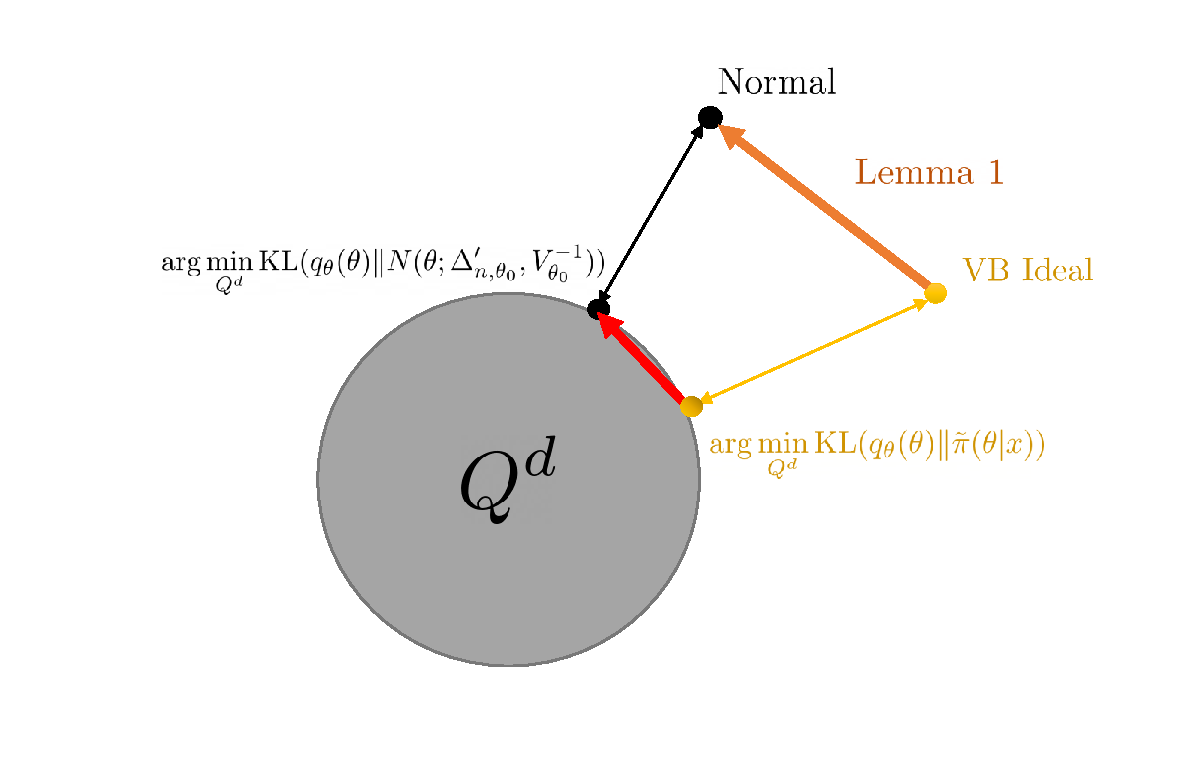
\includegraphics[width = 0.8\linewidth]{graphics/fig1.pdf}
	\label{lemma3fig}
	\caption{Schematic of Lemma \ref{lem3}. The red arrow indicates the convergence implied.}
\end{figure} 

\subsection{Connecting the VB Posterior}

\paragraph{} As mentioned before, we want to derive a BvM result on the global portion of the VB posterior, i.e., $q_{\theta}$. Recall the factorization from equation (8). We can expand the ELBO according to this:
\begin{gather*}
ELBO(q_\theta(\theta)q_z(z)) = \bbE_q[\log(p(\theta,z,x))] - \bbE_q[\log(q_{\theta}(\theta)q_z(z))] \\
= \bbE_{q}[\log(p(x, z|\theta)p(\theta)) - \log(q_{\theta}(\theta)q_z(z))] \\
= \int\int d\theta dz q_\theta(\theta)q_z(z) \log \left( \frac{p(\theta) p(x, z|\theta)}{q_{\theta}(\theta)q_z(z)} \right) \\
= \int d\theta q_{\theta}(\theta) \log \left(\frac{p(\theta)}{q_{\theta}(\theta)} \right) + \int d\theta q_{\theta}(\theta) \int dz q_z(z)\log \left(\frac{p(x,z|\theta)}{q_z(z)} \right)
\end{gather*}
In this form, we can use the strategy of profiling to obtain the optimal distribution $q_{\theta}$, viewing the local factor as a nuisance parameter. That is, if $q_z$ is viewed as fixed, we can derive
$$
q'_{\theta} = \arg\max_{Q^d} ELBO(q_{\theta}(\theta)q_z(z))
$$
%
Now, the factor $q^*_{\theta}$ of the global optimum, i.e., the VB posterior, is obtained simply by taking the maximum value of the ELBO with respect to $q_z$ first. That is,
\begin{equation}
\label{profileELBO}
q_{\theta}^*(\theta) = \arg \max_{Q^d} \left(\sup_{Q^n} ELBO(q_{\theta}(\theta)q_z(z)) \right)
\end{equation}
%
Note the inner supremum still takes on a different value for each $q_{\theta}$. If we denote the profiled ELBO $\sup_{Q^n} ELBO(q_{\theta}(\theta)q_z(z)) = ELBO_p(q_{\theta}(\theta))$, then we can rewrite Equation \ref{profileELBO} as $q_{\theta}^*(\theta) = \arg \max_{Q^d} ELBO_p(q_{\theta}(\theta))$, where
\begin{equation}
ELBO_p(q_{\theta}) = \sup_{Q^n} \int d\theta q_{\theta}(\theta) \left(- \log q_\theta(\theta) \log \left[ p(\theta) \exp \left[ \int dz q_{z}(z) \log\left( \frac{p(x,z|\theta)}{q_z(z)} \right)\right] \right] \right)
\end{equation}
We now have the notation to state the final lemma. 
\begin{lemma}[Lemma 4, \cite{Wang:2019:VBVM}]
	\label{lem4}
	Under some additional technical conditions on the variational densities in $Q^d$ (see exercise 1), we have that for any $q_{\theta}(\theta) \in Q^d$, 
	\begin{equation*}
	ELBO_p(q_{\theta}(\theta)) = -KL(q_{\theta}(\theta)\| \pi^*(\theta|x)) + C_n + o_p(1)
	\end{equation*}
	where $o_p(1)$ indicates that a remainder term converges to $0$ in probability under the probability measures in $Q^d$ and $C_n$ is bounded. 
\end{lemma}

This lemma suggests that the maximizer of the profiled ELBO, i.e., the VB posterior, is also the minimizer of the KL to the VB ideal. In view of Lemma \ref{lem3}, this is a profound result. The proof sketch of this Lemma is appealing and insightful. Notice that the KL divergence is to the VB ideal, which implicitly involves a maximization over $q$, much like the profiled ELBO. We can write the negative KL-divergence as
$$
 -KL(q_{\theta}(\theta)\| \pi^*(\theta|x)) = \int d\theta q(\theta)\log \left( \frac{p(\theta)\exp(M_n(\theta;x))}{q_{\theta}(\theta)} \right) + C_n
$$
%
where the constant $C_n$ is the log of the denominator in the VB ideal. Then,
\begin{equation}
\label{KLlem4}
-KL(q_{\theta}(\theta)\| \pi^*(\theta|x)) = 
\end{equation}
\begin{equation*}
\int d\theta q_{\theta}(\theta) \left(- \log q_\theta(\theta) + \log \left[ p(\theta) \exp \left[ \sup_{Q^n} \int dz q_{z}(z) \log\left( \frac{p(x,z|\theta)}{q_z(z)} \right)\right] \right] \right) + C_n
\end{equation*}
Notice that the term which depends on $q_{\theta}$ differs from the profiled ELBO only by the location of the supremum. Given a $q_{\theta}$, the profiled ELBO implicitly solves the optimization over $q_z$ once. Since the derivation involves solving the joint optimization over both $q_z$ and $q_{\theta}$, it is reasonable to expect that these are simultaneously determined. In equation \ref{KLlem4}, every value of $\theta$ in $q_{\theta}$ can result in a different optimal $q_z$ determining the supremum. To avoid this issue, if $q_{\theta}$ is restricted to be a point mass, then varying $\theta$ does not change the expression and the profiled ELBO and equation \ref{KLlem4} are equivalent. Recall that Lemma \ref{lem1} suggests the VB ideal converges to a point mass. Since the KL divergence between two distributions is infinite if the do not share the same support, the minimizer of the KL divergence to the VB ideal should also converge to a point mass. A portion of the proof is included as Exercise A.1. For a full technical justification, see the appendix in \cite{Wang:2019:VBVM}. 

\subsection{Main Result}
\paragraph{} Prior to stating the main result, we will discuss the chain of implications of the four lemmata above. In Lemma \ref{lem1}, we established the classical BvM result for the rescaled VB ideal, using an extension to misspecified models to account for the variational approximation. This is a precursor to the next two lemmata. We argued heuristically that this meant unscaled VB ideal converges to a point mass. In Lemma \ref{lem2}, we showed that the KL minimizer in the variational family to the VB ideal converges to the point mass at $\theta_0$, i.e., it is consistent. Lemma \ref{lem3} shows that the KL minimizer, or variational approximation to the scaled VB ideal and the variational approximation to a normal are equal in the limit in total variation. In other words, the result from Lemma \ref{lem1} survives the variational approximation on both terms. Finally, Lemma \ref{lem4} states that the maximizer of the ELBO converges to the variational approximation to the VB ideal. Combining with Lemma \ref{lem3} essentially gives the variational BvM result. We now state the main result. 

\begin{theorem}[Variational Bernstein von--Mises Theorem, Theorem 5 \cite{Wang:2019:VBVM}]
	\label{vbvm}
	Let $q^*_{\theta}$ denote the density of the variational approximation $Q^*_{\theta}$ to the posterior distribution of the global latent variables. Suppose the technical conditions of Lemma \ref{lem3} and Lemma \ref{lem4} hold. 
	\begin{enumerate}
		\item (Consistency) The following event occurs almost surely under the true probability measure $P_{\theta_0}$
		\begin{equation*}
		Q^*_{\theta}(\theta) \to \delta_{\theta_0}
		\end{equation*}
		in distribution. 
		\item (Asymptotic Normality) The VB posterior converges to the variational approximation of a normal distribution in total variation. Denote the scaled variational approximation by $\tilde{Q}_{\theta}$ with density $\tilde{q}_{\theta}(\tilde{\theta}) = q^*_{\theta}(\theta_0 + \delta_n\tilde{\theta}) |det(\delta_n)|$. Then, 
		\begin{equation*}
		\| \tilde{Q}_{\theta}  -
		\arg\min_{Q^d} \text{KL}(q_{\theta}(\theta)\| N(\theta; \Delta_{n, \theta_0}', V^{-1}_{\theta_0}))\|_{TV} \to 0
		\end{equation*}
	\end{enumerate}
\end{theorem}
	Recall that normal marginals are independent if and only if its covariance terms are 0. This special fact means that the mean-field variational family includes normal distributions, so long as the covariance matrix is diagonal. Indeed, we can show that
	\begin{equation}
	\label{meanfield}
	\arg\min_{Q^d} \text{KL}(q_{\theta}(\theta)\| N(\theta; \Delta_{n, \theta_0}', V^{-1}_{\theta_0})) = N(\theta; \Delta_{n, \theta_0}', V'^{-1}_{\theta_0})
	\end{equation}
	%
	where $V'_{\theta_0}$ is equal to $V_{\theta0}$ with all off-diagonal terms set to 0. This means that the mean-field scaled VB posterior converges to an uncorrelated normal distribution. The proof of equation \ref{meanfield} can be found in (\cite{Bishop::2006}, section 10.1). 
	
	\paragraph{}Although we restricted the exposition to the mean-field family, the authors emphasize that the results hold as long as lemmata \ref{lem1}-\ref{lem4} are satisfied. In particular, lemmata \ref{lem1} and \ref{lem4} are general in that the proof does not assume the mean-field. Lemma \ref{lem2} holds as long as the variational family at least includes the mean-field. In \cite{Wang:2019:VBVM}, the proof for lemma \ref{lem3} assumes the mean-field family, but it can also be shown for the full-rank Gaussian family. In other words, checking Theorem \ref{vbvm} for a variational family that is extended beyond the mean-field is equivalent to checking lemma \ref{lem3}. 
	

